\documentclass[11pt,a4paper]{article}
\usepackage{cite}
\usepackage{color}
\usepackage{graphicx}
\usepackage{amsmath}
\usepackage[margin=1in]{geometry}
\usepackage{listings}
\usepackage{hyperref}

\title{The DJH INS ROS Package Documentation}
\author{David Hanley, Alex Faustino, David Degenhardt, Tim Bretl}

\begin{document}
\maketitle

\begin{abstract}
	The purpose of this article is to document the approach to the DJH inertial navigation system (INS) ROS package. This package, we anticipate, will be used in a variety of other navigation systems. For example, we design this so that it can be easily used in a visual-inertial odometry system or a magnetic positioning system.
\end{abstract}

\section{Introduction}

The DJH INS ROS package is designed to provide several potentially useful computations to a user as IMU data is received. These include:
\begin{itemize}
	\item IMU data aggregated into sets of Eigen matrices
	\item A state (orientation, position, and velocity) given a set of IMU measurements (aggregated IMU data) and an initial state estimate.
\end{itemize}
Aggregated IMU data can be saved or used by a navigation algorithm or for any purpose. The state estimate is the INS output, which can be used as a prior in navigation systems.

\section{The IMU Aggregator}

One of the functions of the DJH INS is that an INS solution is only computed when requested by the $\texttt{comp\_sol}$ topic. This topic contains a message ($\texttt{compute\_ins.msg}$) created for this package that includes:
\begin{itemize}
	\item $\texttt{Header	header}$
	\item $\texttt{float64	time\_desired}$
	\item $\texttt{bool		stop\_agg}$
	\item $\texttt{float64	start\_time}$
	\item $\texttt{geometry\_msgs/Pose	start\_pose}$
	\item $\texttt{geometry\_msgs/Vector3	start\_vel}$
	\item $\texttt{std\_msgs/Float64MultiArray	aggregatedMatrix}$
\end{itemize}
The $\texttt{time\_desired}$ variable is the time for which an INS solution is desired. The $\texttt{stop\_agg}$ variable is switched to $\texttt{true}$ when it is desired to stop aggregating the data (presumably to then compute an INS solution at $\texttt{time\_desired}$). As the system is running if IMU data is collected with a timestamp at or after $\texttt{time\_desired}$, then that data is saved for use in a matrix with a later $\texttt{time\_desired}$. The $\texttt{start\_pose}$ variable lists the position and orientation of the IMU at the time $\texttt{start\_time}$. The variable $\texttt{start\_vel}$ lists the velocity of the IMU at the time $\texttt{start\_time}$. The aggregated matrix is collected in $\texttt{aggregatedMatrix}$ and published on a topic called $\texttt{aggregate\_imu}$. This topic also consists of a $\texttt{compute\_ins.msg}$ message. The following C++ code shows how to convert the $\texttt{aggregatedMatrix}$ Float64MultiArray message into a regular $n$-by-7 Eigen matrix.
\begin{lstlisting}[frame=single,breaklines] [language=c++]
    /*------- Receive and reform aggregated IMU Matrix -------*/
    // Define a temporary std vector for the aggregated IMU 
    // message data
    vector<double> vec = msg->data;
    // Compute the number of rows in the aggregated matrix
    int sz = vec.size()/7;
    // Create pointer and store memory address of first vector element
    double* ptr = &vec[0];
    // Note: MatrixX7d is defined in aggregator.h
    Map<MatrixX7d>agg_mat(ptr,sz,7);
    /*----- End receive and reform aggregated IMU Matrix -----*/

    // Print Results
    cout << "-----------------------------------------------\n";
    cout << agg_mat << endl;
    cout << "-----------------------------------------------\n";
\end{lstlisting}
The structure of the resulting aggregated matrix is as follows:
\begin{equation*}
	\left[\begin{array}{ccccccc}
		timestamp_1 & accel_{x1} & accel_{y1} & accel_{z1} & gyro_{x1} &  gyro_{y1} & gyro_{z1} \\
		timestamp_2 & accel_{x2} & accel_{y2} & accel_{z2} & gyro_{x2} &  gyro_{y2} & gyro_{z2} \\
		... & ... & ... & ... & ... & ... & ...
	\end{array}\right]
\end{equation*}
Since the DJH INS package is a ROS node, it can interface with some navigation algorithm through ROS topics. Using $\texttt{bare\_bones\_node}$ as an example navigation node (such as a visual-inertial odometry code), the aggregated IMU data can interface with it as shown in Figure \ref{fig:djhinsagg}.


\begin{figure}
	\centering
	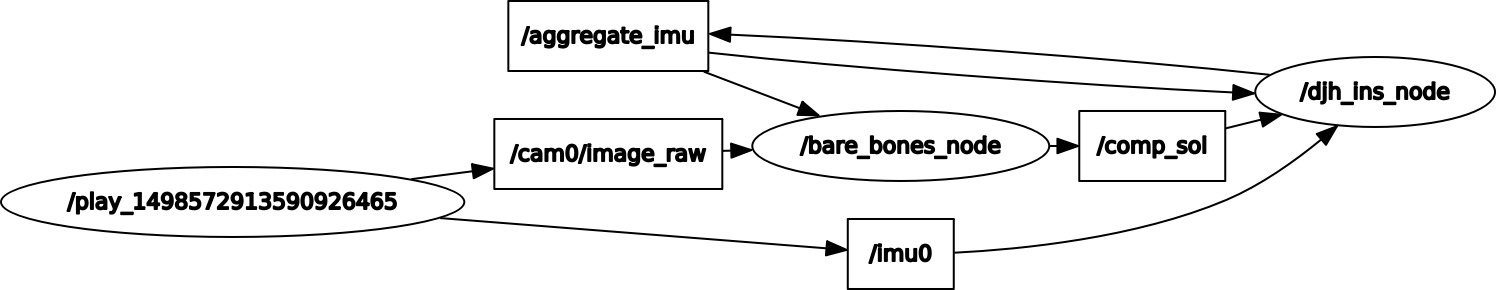
\includegraphics[scale=0.425]{djhinsagg}
	\caption{The DJH INS package receives IMU data and a flag to stop aggregating that IMU data in a matrix. That aggregated data is then published and can be used by both the $\texttt{djh\_ins\_node}$ for computing an INS solution or by some other node (in this case $\texttt{bare\_bones\_node}$) for some other reason.}
	\label{fig:djhinsagg}
\end{figure}

\section{The IMU Model and Corrector}

The elements of the aggregated matrix are corrected for fixed scale factors ($S_g$ and $S_a$), cross-coupling effects ($M_g$ and $M_a$), and biases ($B_{fg}$ and $B_{fa}$). These parameters (since they are fixed) are set in a parameter file called $\texttt{IMUmodel.yaml}$. We also assume that the navigation algorithm can potentially estimate some bias online ($B_g$ for the gyroscopes and $B_a$ for the accelerometers). Therefore, we have set up a subscriber to a ROS topic called $\texttt{bias\_est}$ which contains a $\texttt{std\_msgs::Float64MultiArray}$ message. The first three elements of the message are assumed to correspond to the x, y, and z-axis accelerometer biases respectively. The second three elements of the message are assumed to correspond to the x, y, and z-axis gyroscope biases respectively. Equations \ref{fig:gyrocorrect} and \ref{fig:accelcorrect} show how we use measurements from the gyroscopes, $\omega$, and accelerometers, $a_{sf}$, to compute corrected gyroscope, $\tilde{\omega}$, and accelerometer, $\tilde{a}_{sf}$, data. Figure \ref{fig:withonlinebias} shows the same information as Figure \ref{fig:accelcorrect}. However, now ROS topics relevant for IMU error correction is also included.

\begin{equation}
	\tilde{\omega} = (1 + S_g)\omega + M_g \omega + B_{fg} + B_g
	\label{fig:gyrocorrect}
\end{equation}

\begin{equation}
	\tilde{a}_{sf} = (1 + S_a)a_{sf} + M_a a_{sf} + B_{fa} + B_a
	\label{fig:accelcorrect}
\end{equation}

\begin{figure}
	\centering
	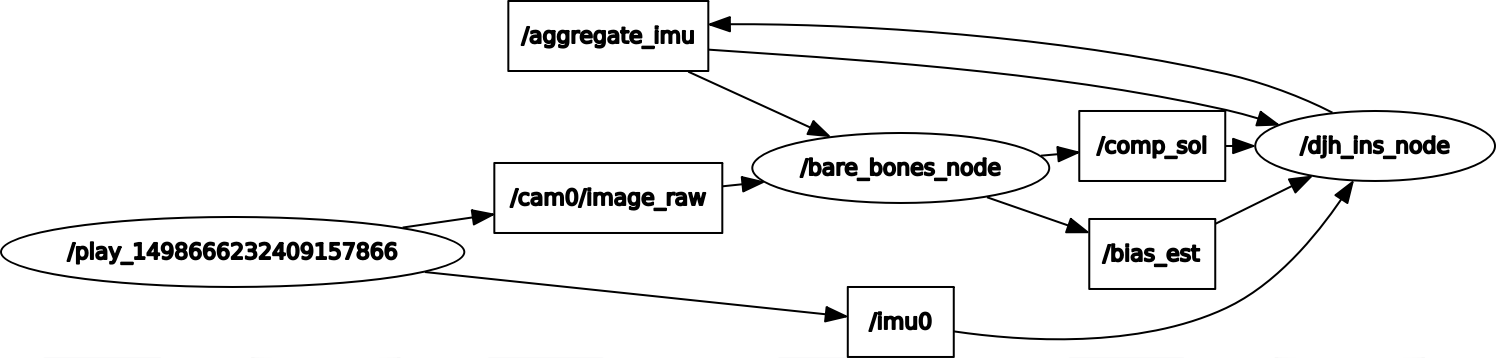
\includegraphics[scale=0.42]{withonlinebias}
	\caption{This ROS graph shows all the ROS topics associated with aggregating IMU data and with correcting IMU measurements.}
	\label{fig:withonlinebias}
\end{figure}

\section{Quaternion Math Library}

Our INS code makes significant use of the C++ library Eigen (\url{http://eigen.tuxfamily.org}). However, we do not make use of Eigen's quaternion functionalities. This is because we use a JPL convention for quaternions. More information on the JPL convention can be found at \cite{Trawny:2005,Barfoot:2011,Wie:2008}. Therefore, we create our own quaternion math class call $\texttt{QuatMath}$ which performs the following functions on JPL-style quaterions:
\begin{itemize}
	\item[1] Normalize the Quaternion
	\item[2] Compute the Angle of Rotation
	\item[3] Perform Quaternion Multiplication
	\item[4] Compute the Quaternion Inverse
	\item[5] Create a Rotation Matrix from a Quaternion
	\item[6] Convert Rotation Matrix to a Quaterion.
\end{itemize}
Note that to convert from a JPL quaternion to a Hamilton quaternion one must simply apply the following transformation
\begin{equation}
	q^{H}  = \left[\begin{array}{cccc} q^{JPL}_4 & -q^{JPL}_1  & -q^{JPL}_2  & -q^{JPL}_3 \end{array}\right]^T.
\end{equation}

\section{Integration Algorithms and Implementation}

To select our INS integration scheme, we conducted a quick survey of methods used in visual-inertial odometry algorithms:
\begin{itemize}
	\item Fourth-order Runge-Kutta integration \cite{Mirzaei:2008,Hesch:2014,Keivan:2015,Kelly:2011}
	\item Fourth-order Runge-Kutta integration for attitude and Simpson integration for position and velocity \cite{Li:2013}
	\item Euler integration \cite{Jones:2011}
	\item Preintegration \cite{Artal:2017}
\end{itemize}
Based on this, we decided to use a standard fourth-order Runge-Kutta method to compute our INS results. Note that for batch optimization methods, preintegration methods are preferable because aggregated IMU measurements do not need to be saved. More over, methods from Savage \cite{SavageP1:2007,SavageP2:2007} may be computationally more efficient and may better handle the effects of coning, sculling, and scrolling. However, we leave such methods for future work.

\subsection{Gravity Model}
The gravity model we use is described in \cite{Titterton:2004}. Gravity magnitude (in $m/s^2$) determined by latitude is
\begin{equation}
	g(0) = 9.780318(1+5.3024\times 10^{-3} \sin^2 L - 5.9 \times 10^{-6} \sin^2 2L)
\end{equation}
and the magnitude due to height is determined by
\begin{equation}
	g(h) = \frac{g(0)}{\left(1 + h/R_0\right)^2}
\end{equation}
where $h$ is the altitude in meters, $L$ is the latitude in radians, and $R_0$ is the Earth's mean radius in meters. This is applied to a vector a vector as $\mathbf{g} = \left[\begin{array}{ccc} 0 & 0 & g(h)\end{array}\right]^T$ in the NED frame. Finally, we apply the Coriolis effect due to Earth's rotation to compute the entire plumb-bob gravity vector of the IMU frame ($l$) in the NED frame ($n$)
\begin{equation}
	\mathbf{g}^n_l = \mathbf{g} - \frac{\Omega^2\left(R_0 + h \right)}{2}\left(\begin{array}{c} \sin 2L \\ 0 \\ 1 + \cos 2L \end{array} \right)
\end{equation}
where $\Omega$ is the rotation rate of the Earth in radians per second. Note that we created a parameter file called \texttt{Earthparam.yaml} which contains the following parameters:
\begin{itemize}
	\item The latitude of the location
	\item The altitude of the location
	\item The Earth's mean radius
	\item The rotation rate of the Earth.
\end{itemize}
Thus if the Coriolis effect must be ignored, then the rotation rate of the Earth can be set to zero. It is here also assumed that in the applications in which DJH INS will be used, the latitude or altitude of the system will not change dramatically enough during operation for the gravity model to be significantly impacted. 

\subsection{Equations of Motion}
The equations of motion we use to describe the motion of the IMU are
\begin{align}
	\dot{q} & = \frac{1}{2}\Omega(\tilde{\omega}) q \\
	\dot{p} & = v \\
	\dot{v} & = C(q)\tilde{a}_{sf} + \mathbf{g}^n_l
\end{align}
where $q$ is the orientation, $p$ is the position, and $v$ is the velocity of the IMU in the NED frame. The matrix $\Omega(\tilde{\omega})$ is the appropriate $4\times 4$ matrix created from corrected gyroscope measurements $\tilde{\omega}$. The $3 \times 3$ matrix $C(q)$ is the rotation matrix generated from the quaternion $q$.

\subsection{Runge Kutta Integration and Run Time}
Expressing our equations of motion as $\dot{x} = f(x)$, we compute a classical Runge-Kutta solution as
\begin{align}
	k_1 & = f(x_i) \\
	k_2 & = f(x_i + \frac{\Delta t}{2}k_1) \\
	k_3 & = f(x_i + \frac{\Delta t}{2}k_2) \\
	k_4 & = f(x_i + \Delta t k_3) \\
	x_{i+1} & = x_i + \frac{\Delta t}{6}\left(k_1 + 2 k_2 + 2 k_3 + k_4\right) 
\end{align}
where $x_i$ is the state at step $i$ and $\Delta t$ is the time between step $i$ and $i+1$. We update the state estimate by solving the Runge-Kutta equations between each IMU measurement between our start and finish time stamps.

The INS result is publish on a ROS topic called $\texttt{ins\_result}$ as a $\texttt{compute\_ins.msg}$ message. In this topic, the $\texttt{start\_time}$ and $\texttt{time\_desired}$ are both set to the $\texttt{time\_desired}$ used to compute the INS solution. The final full INS ROS package graph is shown in Figure \ref{fig:finalgraph}.

Note that we tested our algorithm on the EuRoC dataset \cite{Burri:2016}. This has a camera that provides images at 20 Hz and an IMU that provides measurements at 200 Hz. We request an INS solution every time we receive an image. It requires on our test computer (which uses an i7 processor with 16 GB of RAM) approximately 0.002 seconds to compute an INS solution. Note that this is faster than the frame rate of the camera and that IMU data collection does not stop while we compute and INS solution (since these are different processes). Note also that if we received a faster camera, we would have fewer IMU measurements, so the runtime of the INS solution will be much faster (since the Runge-Kutta calculation requires the bulk of the time).

\begin{figure}
	\centering
	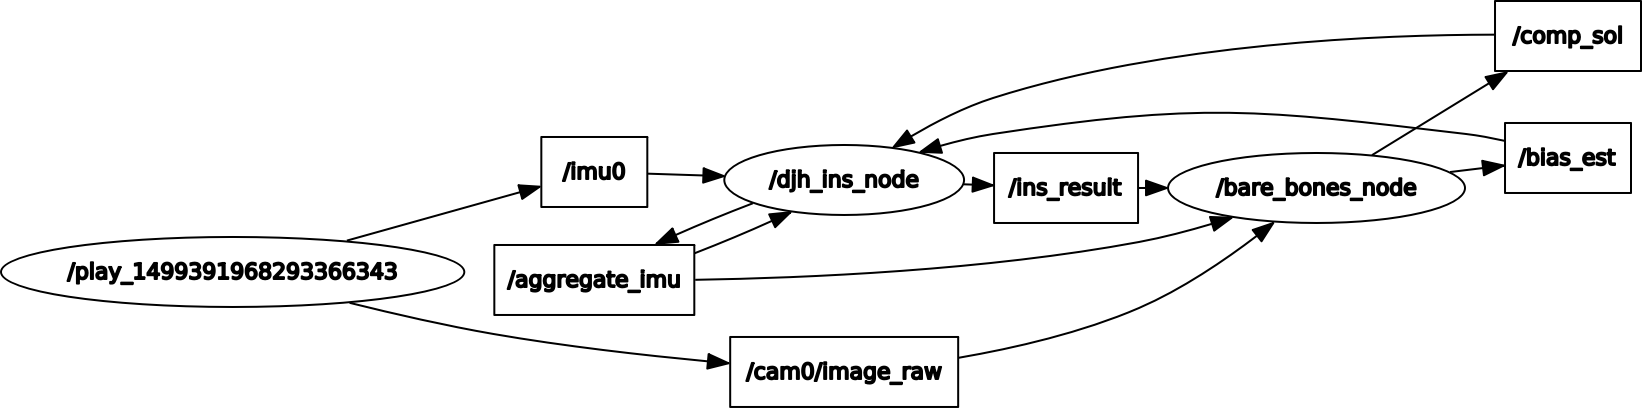
\includegraphics[scale=0.37]{finalgraph}
	\caption{This ROS graph shows all the ROS topics associated with the DJH INS package.}
	\label{fig:finalgraph}
\end{figure}

\section{Test Cases}

\subsection{The Spin-Cone Truth Model}

As a first test case, we use the Spin-Cone Model described by \cite{Savage:2009}. This model tests the attitude integration algorithms against a known closed-form solution. This models spins about one axis and precesses about another as shown in Figure \ref{fig:spincone}. The ground truth is determined by Euler angle equations
\begin{align}
	\phi & =\left(\omega_s - \omega_c \cos \beta\right) t + \phi_0 \\
	\theta & = \frac{\pi}{2} - \beta \\ 
	\psi & = -\omega_c t.
\end{align}
We assume that $a_{sf} = 0$. The gyroscope measurements $\omega^B_{iB}$ are determined by the equations
\begin{align}
	\omega^R_{iB}(t) & = \left[\begin{array}{c}\omega_s t \\ \frac{\omega_c\sin\beta}{\omega_s-\omega_c\cos\beta}\left(\cos\phi - \cos\phi_0\right) \\ \frac{-\omega_c \sin\beta}{\omega_s-\omega_c\cos\beta}\left(\sin\phi-\sin\phi_0\right)\end{array}\right] \\
	\omega^B_{iB}(t) & = C^B_R\omega^R_{iB}(t).
\end{align}
Here parameters $\omega_s$, $\omega_c$, $\beta$, $\phi_0$, and the rotation matrix $C^B_R$ are chosen by the user. The closed form solution is described by the equations
\begin{align}
	C^N_R & = \left[\begin{array}{ccc} c_\theta c_\psi & -c_\phi s_\psi+s_\phi s_\theta c_\psi & s_\phi s_\psi + c_\phi s_\theta c_\psi \\
	c_\theta s_\psi & c_\phi c_\psi + s_\phi s_\theta s_\psi & -s_\phi c_\psi + c_\phi s_\theta s_\psi \\
	-s_\theta & s_\phi c_\theta & c_\phi c_\theta \end{array}\right] \\
	C^N_B & = C^N_R C^R_B.
\end{align}

\begin{figure}
	\centering
	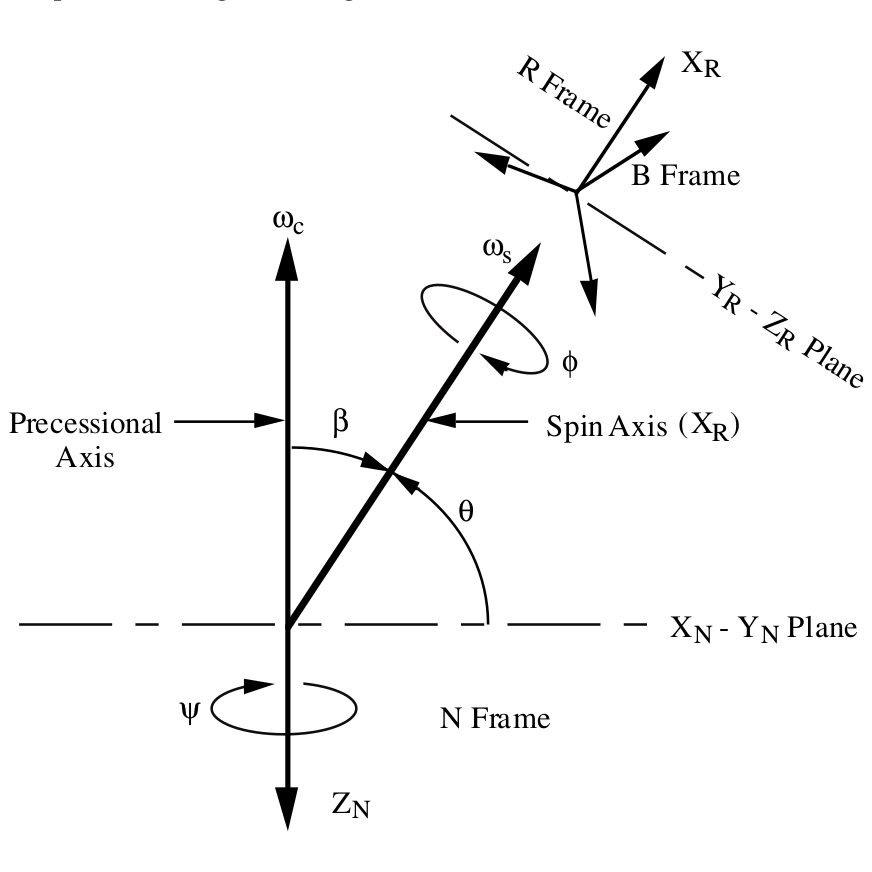
\includegraphics[scale=0.3]{spincone}
	\caption{The spin-cone test model.}
	\label{fig:spincone}
\end{figure}

\section{Future Work}

In the future, we would like to make significant changes to this package. First, we would like to add preintegration as part of our packag\cite{Forster:2017,Forster:2015,Eckenhoff:2016}. Second, we would like to include as many performance analysis test cases (as described in \cite{Savage:2009}) as possible.

\bibliographystyle{IEEEtran}
\bibliography{IEEEabrv,references}

\end{document}